%--------------------------------------------------
%	Chapter 5. GNN Pattern Recognition Algorithm
%--------------------------------------------------

\chapter{Graph Neural Network Pattern Recognition Algorithm}\label{chapter-5}

Once compatible hit-pairs have been established, they can be used to build a graph network to represent a particle collision event. This chapter presents a novel pattern recognition algorithm utilising GNN architectures to prune connections in such a network, in order to reconstruct tracks in a silicon based Pixel detector. The application is focused on the Pixel detector, with the aim that the approach will serve as a sophisticated track seeding technique for Pixel hits and form preliminary track candidates. These seeds can be extended into the Strips using standard track following. Such an approach could be efficient for saving computational resources if the GNN does not produce large proportions of fake tracks. The ultimate aim of this work is to develop a realistic algorithm for fast track reconstruction that can be deployed in future high-luminosity phases of particle detector experiments. This work was presented at the 2022 Connecting the Dots (CTD) conference at the University of Princeton USA and is currently under review for publication in the Springer Journal: Computing for Software and Big Science \cite{Lad_2023_gnn}. Sections \ref{gnn-algorithm-overview} to \ref{gnn-kf-implementation} present an overview and detailed breakdown of each stage of the algorithm and Section \ref{gnn-application-toy-model} illustrates a simple application on a toy model.



\section{Algorithm Overview}
\label{gnn-algorithm-overview}
The GNN based pattern recognition algorithm is considered as an iterative mixture reduction task, that allows deactivating incompatible connections (GNN edges termed as outliers) in order to improve track parameter estimates and iteratively extract track candidates. 

Individual hits or clusters of hits are modelled as graph nodes and track segments are modelled as graph edges. Once the graph network is constructed, each edge is modelled as a Gaussian state in order to approximate the local track state probability density. Therefore, each node is initialised with a Gaussian mixture of track states, local to its neighbourhood of connections.

After initialisation, the network evolves iteratively, where an iteration is made up of three main stages illustrated in Figure \ref{fig:flowchart}. The first stage comprises of Gaussian Mixture Reduction (GMR). This involves a traditional ML approach, whereby compatible Gaussian states are grouped together using clustering techniques and outlier states can be identified. This stage is followed by information aggregation by leveraging message passing between nodes in a given neighbourhood. The compatibility of neighbouring states can be assessed via extrapolation, in order to improve local track parameters using neighbourhood information. The third stage involves updating the network state at each node, as certain connections are deactivated. After stages one and two a graph splitting algorithm is applied to identify good track candidates, and if discovered they are extracted via the KF. 

Unlike traditional methodologies whereby Multi-Layered Perceptrons (MLPs) are employed for deep learning strategies, the proposed GNN leverages simplified KFs embedded in the network and are used for two main purposes. Firstly, the KF is used as a mechanism for information propagation, in order to iteratively improve the precision of track parameters. Secondly, the KF is used in extraction of track candidates compatible with particle motion model. This allows the model to efficiently exploit a prior knowledge about charged particle dynamics as the network evolves.

The excitation and inhibition rules of individual edge connections are designed to facilitate the “simple-to-complex” approach for “hits-to-tracks” association, such that the network starts with low hit density regions of an event and gradually progresses towards more complex areas. As the network evolves, the uncertainty in local track orientation decreases until there are no more track candidates that fulfil the criteria for a good track. This is the end state of the network where isolated nodes, track fragments and unresolved ambiguities will remain.

\begin{figure}[htbp]
    \centering
    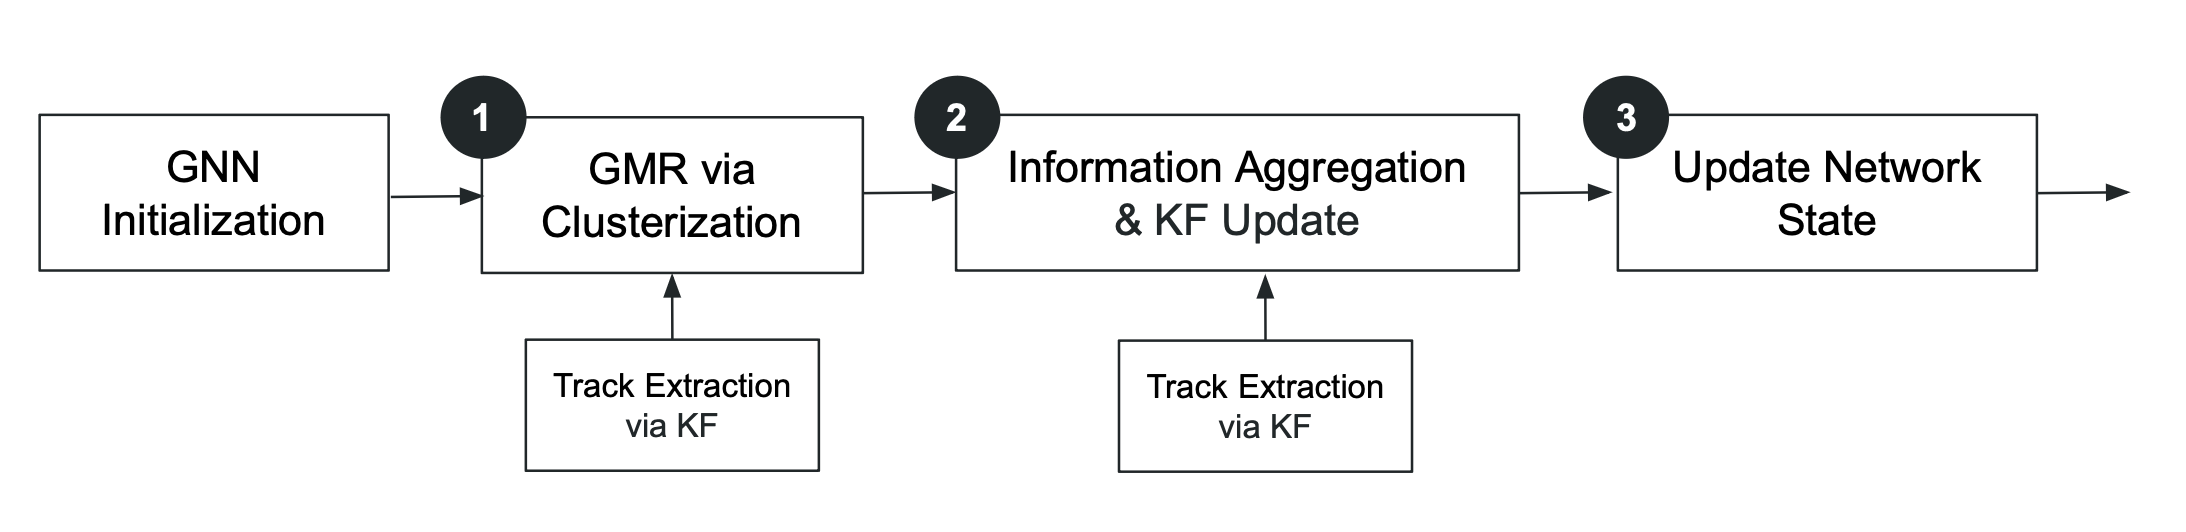
\includegraphics[width=0.98\textwidth]{images/5-gnn-algorithm/gnn-workflow.png}
    \caption{Flow chart illustrating all stages making up an iteration of the GNN-based algorithm. After each stage, a Kalman filter is applied in order to iteratively extract candidates. After stage three, a further Gaussian Mixture Reduction (GMR) stage would be applied repeating the iterations.}
    \label{fig:flowchart}%
\end{figure}



\section{Network Initialization}
\label{gnn-network-initialization}

\begin{itemize}
\item Using networkX python package?
\item Event conversion and graph construction nodes and edges?
\item Gaussian mixture equations
\item nodes represents hits (or combinations of hits) and edges represent the edge connections between hit-pairs
\item Track State equations, covariances, derivations, r-z plane and transverse plane
\item edges having priots and weights (strength and compatibility) - because of Gaussian mixture
\item edges act as bidrectional conduits - passing information both ways between nodes
\end{itemize}

\subsection{Track State Estimates}
\begin{itemize}
\item In both xy and rz planes, joint track state estimate
\item parabolic model - in local coordinate system of node itself
\item rz joint vector - tau parameter, inverse track inclination
\item how were the covariances dervied and the sigma errors chosen
\end{itemize}

\subsection{Molière Theory of Multiple Scattering}
\begin{itemize}
\item highland formula and handling the error/effects due to multiple scattering for the barrel and endcap in slightly different ways
\end{itemize}
% moliere theory links:
%https://gray.mgh.harvard.edu/attachments/article/337/Techniques%20of%20Proton%20Radiotherapy%20(06)%20Multiple%20Scattering.pdf
%https://pdg.lbl.gov/2005/reviews/passagerpp.pdf



\section{Gaussian Mixture Reduction}
\begin{itemize}
    \item GMR theory
    \item Clustering, KL divergence
    \item Mahalanobis distance and merging of states
    \item training the optimal threshold using an SVM
    \item feeding in using a fast look-up table
\end{itemize}



\section{Information Aggregation}
\begin{itemize}
    \item Information propagation via Message Passing
    \item Extrapolation and Validation
    \item Linear and Parabolic model - 2 different extrapolations for xy componenets of state vector and rz componenet, illustrations here
    \item Kalman Filter Update, OU process for correlated noise
\end{itemize}



\section{Updating Network State}
\label{gnn-updating-network-state}

As the network evolves and certain connections are deactivated, the local track parameter estimates for each node changes. Therefore, the corresponding edge component's $w_{ij}$ are updated. For an edge connection between nodes $i$ and $j$, the updated edge weights $\widetilde{w}_{ij}$ stated in Eq. \eqref{eqn:weights} are computed using the normalised Gaussian measurement likelihood given by Eq. \eqref{eqn:likelihood}. The denominator $\sum_{k}w_{ik}\beta_{ik}$ is the summation of the product of weights and likelihoods in a neighbourhood for a given node $i$. The updated weights $\widetilde{w}_{ij}$ are also divided by the number of detector layers on either side of its neighbourhood $N_S$, in order to account for the probability that a track passing through node $i$ was detected at layer $L$. For a given node, if any $\widetilde{w}_{ij} < 0.1$, these edge connections are automatically deactivated as the likelihood of compatibility of this incoming track state is extremely low. This forms an additional part of the mechanism for edge activation and deactivation. After this update is complete, the iterations repeat and a further GMR would be performed on updated track states. 

\begin{equation}
\beta_{ij} = (2 \pi \lvert S_{ij} \rvert )^{-1/2}  e^{-\Delta \chi^{2}_{ij} / 2}
\label{eqn:likelihood}
\end{equation}

\begin{equation}
\widetilde{w}_{ij} = \frac{1}{N_S} \frac{w_{ij}\beta_{ij} p_i}{\sum_{k}w_{ik}\beta_{ik}}
\label{eqn:weights}
\end{equation}



\section{Track Extraction}
\begin{itemize}
    \item CCA
    \item criteria for a good track candidate
    \item Implementation of KFs/ KF track fit
    \item Merging Close Proximity Nodes
    \item Community Detection
\end{itemize}
%Community Detection: divides nodes into various clusters based on edge structure. It learns from edge weights, and distance and graph objects similarly. 



\section{Implementation of KFs}
\label{gnn-kf-implementation}

\begin{itemize}
\item emphasis on the use of KFs both in information aggregation stage and in track extraction, both are implemented in different ways, is a useful and unique part to this algorithm
\end{itemize}



\section{Application and Performance on a Simple Toy MC Model}
\label{gnn-application-toy-model}

% The excitation and inhibition rules of individual GNN nodes will be designed to facilitate the “simple-to-complex” approach for “hits-to-tracks” association, such that the network starts with relatively “easy” areas of an event (low hit density) and gradually progresses towards more complex areas (high hit density). 

\begin{itemize}
\item Application on a simple toy mc model and heat network - track extracted and metrics
\end{itemize}



\section{Conclusions}
